% User-authorized systems result, 8 September 2026; not a new training experiment.
% Evidence: ../../runs/029-2026-09-07-pythia14m-matched-kernel-retrospective/
% observations/06-implementation-and-claim-audit.md and observations/05-kernel-autoresearch-and-rmodel.md.
% Independent audit: that run's 19_audit_evidence.py and results/implementation-audit-001.json.
% Figure generator: that run's 18_paper_summary.py --revision 3.
% Implementation, numerical bounds, provenance and limitations: kernel-implementation.md.
% Attention discussion: Observation03 counters/ablations; longer-T claim is an untested hypothesis.
\subsection{Realizing sparsity with specialized inference kernels}
\label{sec:kernel-autoresearch}

Does training-induced sparsity translate into faster execution when kernels
are specialized to exploit it? We examine a human-guided coding-agent search
using Codex, with recorded default model \emph{gpt-6-astra}.\footnote{The
retained configuration identifies the default model, not the model served
for every request; this is one assisted development trajectory.}
A matched retrospective reevaluates 42 eligible Pythia-14M kernel proposals
against the same-checkpoint native PyTorch/SDPA CUDA-graph baseline on one
RTX5090. The workload is BF16, batch one, and 2,048-token uncached causal
inference with full vocabulary logits. Timings use 64 fixed validation
inputs in three fresh processes; numerical qualification covers all
338 complete validation blocks.

The final implementation combines fused normalization and RoPE with
zero-fragment bypass and sparse-row projection paths.
The qualified incumbent reaches $1.78\times$ speedup on the fixed search
checkpoint (Figure~\ref{fig:kernel-autoresearch}, left). The final kernel
qualifies on all 35 retained checkpoints; its geometric mean speedup is
$1.25\times$. Across these checkpoints, speedup has a positive association
with $\Smodel$ (right; unweighted OLS $R^2=0.781$), rather than a strictly
monotonic scaling law.

An ablation retaining the fusion but disabling sparse paths separates part
of their contribution: enabling those paths adds $31.1\%$ acceleration at
the search checkpoint and $5.6\%$ geometrically averaged over the cohort,
helping 19 of 35 checkpoints.

Attention skipping is active but not profitable at $T=2{,}048$: at the search
checkpoint, it bypasses $58.0\%$ of QK and $67.2\%$ of PV tensor-core
matrix-multiply--accumulate operations. Nevertheless, disabling attention
skipping improves all 35 checkpoints (geometric mean $1.267\times$ versus
$1.250\times$), locating the positive net sparse-path contribution in the
projections. Longer uncached sequences could change this trade-off: attention
products grow quadratically with $T$, whereas projection and LM-head products
grow linearly for fixed architecture (Equation~\ref{eq:denominator}). This
does not guarantee a crossover, since zero checks and control also recur
within attention tiles, and zero-fragment structure may change. Longer-$T$
profitability remains untested and requires length-adapted kernels, fresh
numerical qualification and matched timing; this implementation supports only
$T=2{,}048$.

Thus, this case demonstrates that an agent-assisted implementation can
realize inference gains from training-induced activation sparsity, while
also showing that fusion and sparse-path overhead matter. It does not
establish equal-quality gains, transfer to cached decoding or other hardware,
or superiority over human kernel development.

\begin{figure}[htbp]
\centering
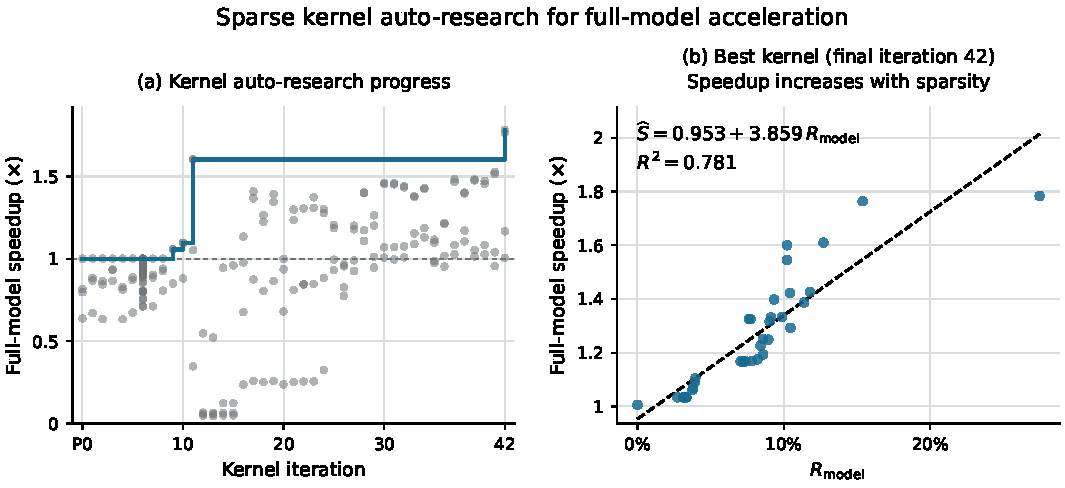
\includegraphics[width=\linewidth]{../../runs/029-2026-09-07-pythia14m-matched-kernel-retrospective/figures/04-kernel-autoresearch-and-rmodel.pdf}
\caption{Matched kernel auto-research and sparsity-dependent acceleration.
(a) Gray points show 214 timed candidate/checkpoint comparisons, including
74 numerical failures; they are not all valid accelerations. The blue line
tracks the best qualified incumbent on the fixed A7-OL1, $\kappa=0.5$
checkpoint, initialized at native $1\times$. P0 is a separate comparator,
not an iteration; two unsupported comparisons have no timings.
(b) The final historical kernel, K050 at iteration 42, evaluated on all
35 checkpoints. The dashed line is OLS with an estimated intercept.
The figure's $R_{\mathrm{model}}$ denotes $\Smodel$: ticks are percentages,
while the fitted equation uses fractions. Both axes are linear; panel (b)
uses a restricted speedup range. Checkpoints differ in topology, weights
and loss, so the association does not isolate a causal sparsity effect.}
\label{fig:kernel-autoresearch}
\end{figure}
